\documentclass[tikz]{standalone}
\usetikzlibrary{automata,positioning}
\begin{document}

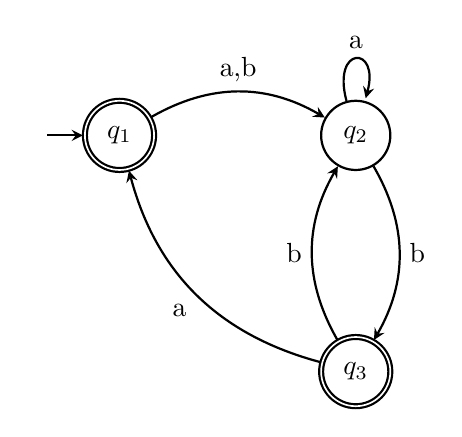
\begin{tikzpicture}[>=stealth,node distance=3cm,on grid,auto, thick, initial text=] 
  \node[state, initial, accepting] (q_1) {$q_1$};
  \node[state] (q_2) [right=of q_1] {$q_2$};
  \node[state, accepting] (q_3) [below=of q_2] {$q_3$};

  \path[->]  (q_1) edge [bend left] node {a,b} (q_2)
  (q_2) edge [loop above] node {a} (q_2)
  (q_2) edge [bend left] node {b} (q_3)
  (q_3) edge [bend left] node {a} (q_1)
  (q_3) edge [bend left] node {b} (q_2);
\end{tikzpicture}
\end{document}
